\chapter{Objetivos}
\label{chap:objetivos}

\drop{E}n primer lugar se va a exponer el objetivo principal del \ac{TFG}. Y en segundo lugar qué subojetivos se han planteado de tal forma que se pueda seguir una buena metodología de trabajo debido a la correcta modularización del proyecto. 

\section{Objetivo principal}\label{ObjetivoPrincipal}

El objetivo principal del proyecto es conseguir que un vehículo llegue desde un punto de origen a un punto de destino esquivando los obstáculos que aparezcan en el escenario en tiempo real.

Para llegar a cumplir este objetivo es necesario plantear distintos subobjetivos de tal forma que se cubran todas las necesidades para llevar a cabo nuestro proyecto.

\section{Objetivos específicos}\label{ObjetivosEspecíficos}

Como objetivos específicos del sistema podemos encontrar los siguientes:

\begin{definitionlist}
\item[Subojetivo \ref{sec:DetecciónObstáculos}: \nameref{sec:DetecciónObstáculos}] Distinguir los obstáculos del entorno.
\item[Subobjetivo \ref{sec:DetecciónVehiculo}: \nameref{sec:DetecciónVehiculo}] Distinguir el vehículo frente a los demás objetos y calcular su posición en el entorno.
\item[Subobjetivo \ref{sec:CalculoTrayectoria}: \nameref{sec:CalculoTrayectoria}] Calcular la trayectoria por la que debe avanzar el vehículo.
\item[Subobjetivo \ref{sec:GenerarMovimientos}: \nameref{sec:GenerarMovimientos}] Traducción de los datos de la trayectoria en movimientos.
\item[Subobjetivo \ref{sec:ComunicaciónVehículo}: \nameref{sec:ComunicaciónVehículo}] Comunicar el coche con el sistema.
\item[Subobjetivo \ref{sec:MovimientoVehículo}: \nameref{sec:MovimientoVehículo}] Realizar movimientos con el vehículo de manera inalámbrica y automática.
\item[Subobjetivo \ref{sec:TiempoReal}: \nameref{sec:TiempoReal}] Conseguir que el sistema funcione en tiempo real.
\end{definitionlist}

\subsection{Detección de obstáculos}\label{sec:DetecciónObstáculos}

Se deben detectar los obstáculos que aparezcan en el escenario en función del tiempo. Teniendo en cuenta que el funcionamiento del sistema está pensado para que el coche esquive objetos en tiempo real, se necesita implementar un algoritmo que detecte los obstáculos que aparecen y desaparecen en el entorno. Es decir, el escenario sobre el que se desarrolla la ejecución del proyecto es fijo. Por lo que este algoritmo debe comprobar si se ha producido algún cambio en el entorno para delimitar la posición de los objetos.

\begin{figure}[htbp]
 \centering
  \subfloat[Inicial]{
   \label{fig:Laboratorio}
    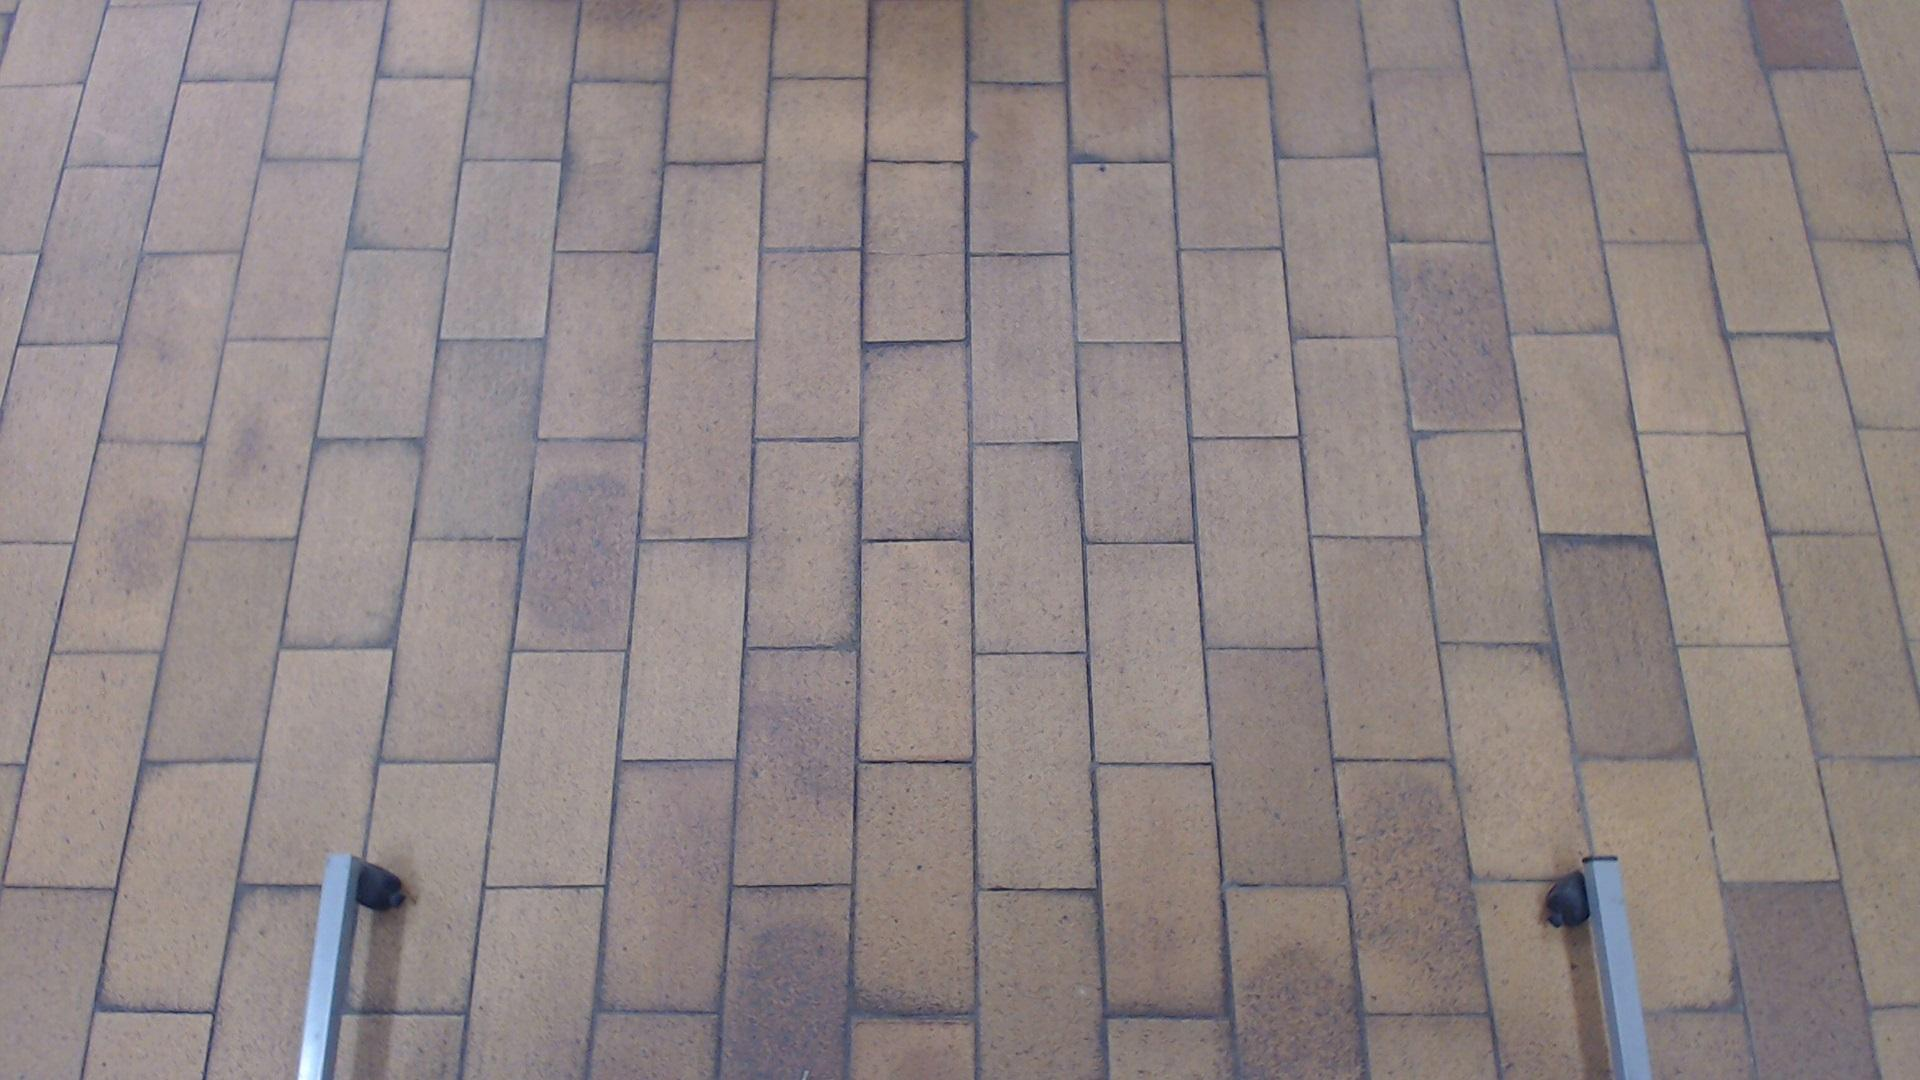
\includegraphics[width=0.49\textwidth]{./figures/Laboratorio.jpeg}}
  \subfloat[Nuevo]{
   \label{fig:LaboratorioObjetos}
    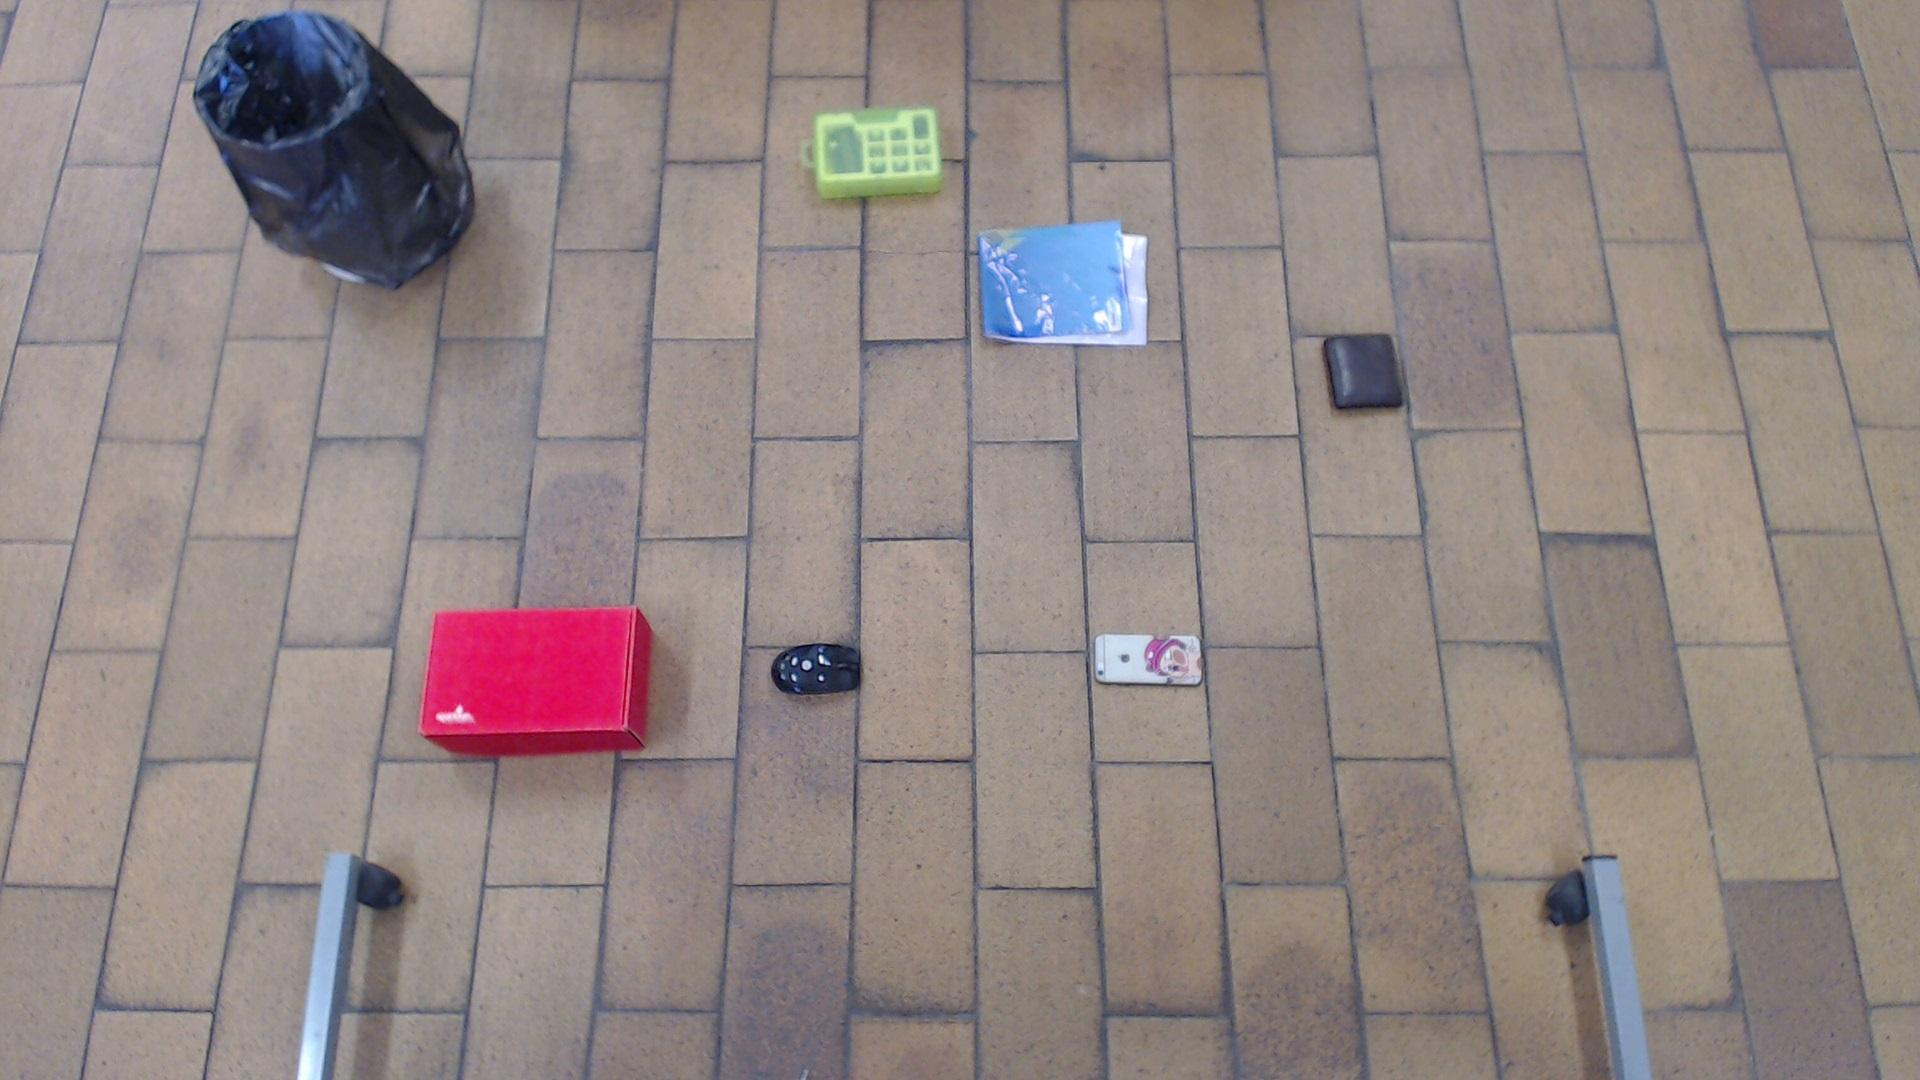
\includegraphics[width=0.49\textwidth]{./figures/LaboratorioObjetos.jpeg}}
 \caption{Estados del entorno del proyecto}
 \label{fig:EstadosLaboratorio}
\end{figure}

\subsection{Distinción y cálculo de posición del vehículo}\label{sec:DetecciónVehiculo}

Se requiere un algoritmo que detecte la posición del vehículo en el escenario para poder introducir las coordenadas desde las que comenzar el cálculo de la trayectoria que debe seguir el vehículo. Para ello, se debe detectar un rasgo identificativo que diferencie al coche de los demás objetos.

\begin{figure}[htbp]
 \centering
    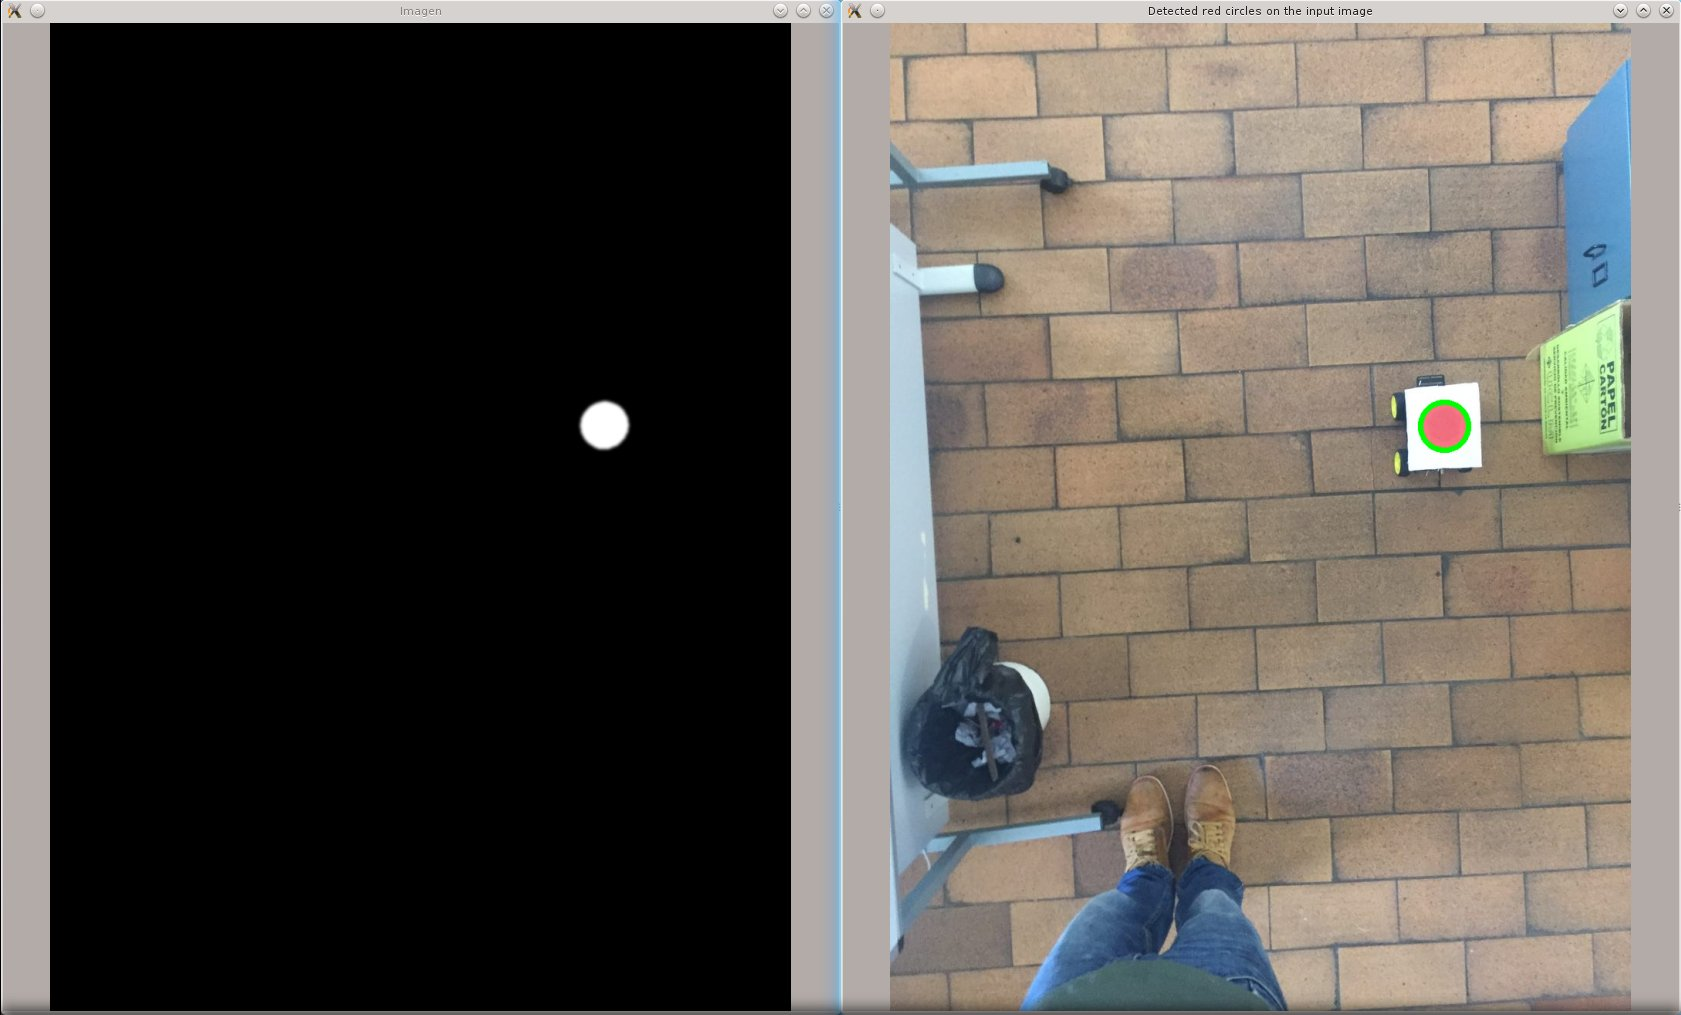
\includegraphics[width=0.8\textwidth]{./figures/deteccionvehiculo.jpeg}
 \caption{Ejemplo de detección de la posición del vehículo en el entorno.}
 \label{fig:EstadosLaboratorio}
\end{figure}

\subsection{Cálculo de trayectoria}\label{sec:CalculoTrayectoria}

Es necesaria la inclusión de un algoritmo en el sistema que calcule la trayectoria que debe seguir el vehículo para evitar colisionar con los posibles obstáculos del entorno. Como este proyecto está orientado al funcionamiento en tiempo real, el sistema deberá calcular una nueva ruta cada vez que el entorno cambie. Por ello, es necesario que el algoritmo no demore mucho tiempo.

\begin{figure}[htbp]
 \centering
  \subfloat[Entorno Prueba]{
    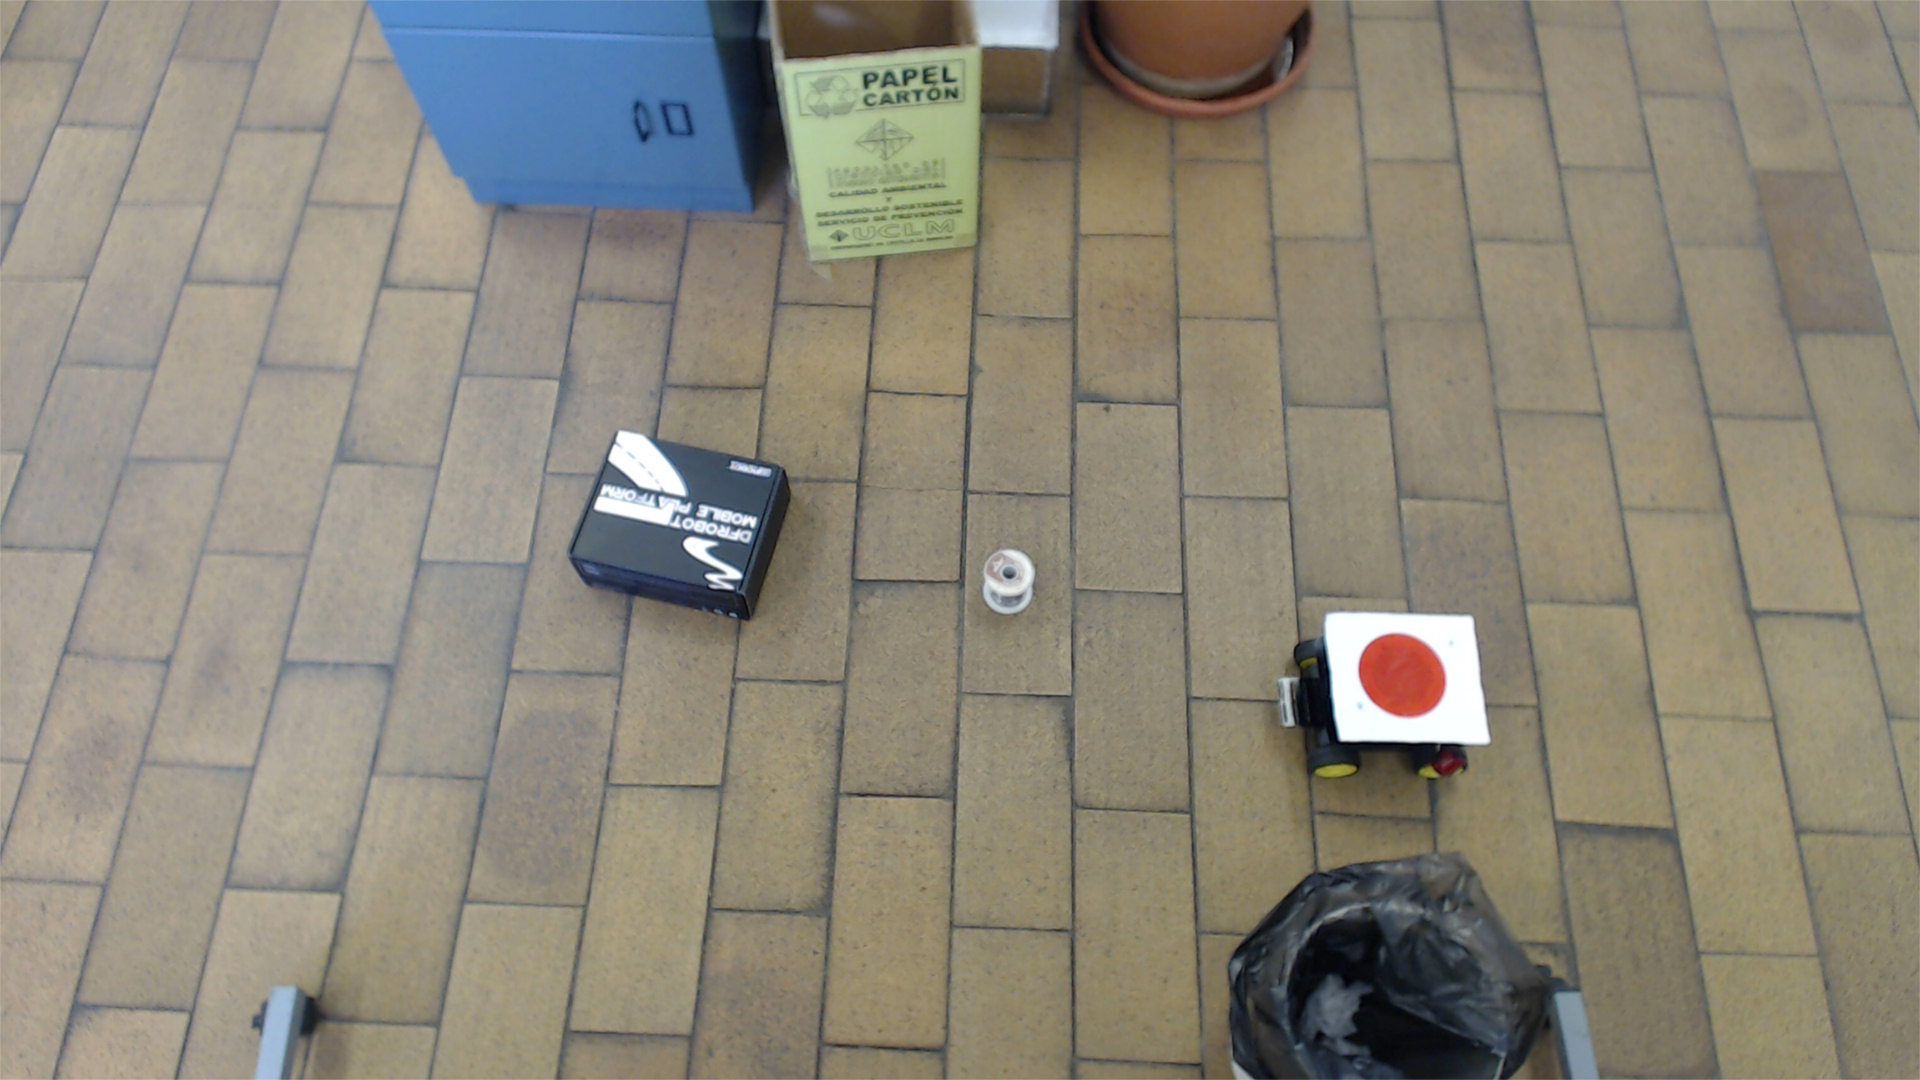
\includegraphics[width=0.49\textwidth]{./figures/scenarioVehicle.jpg}}
  \subfloat[Resultado]{
    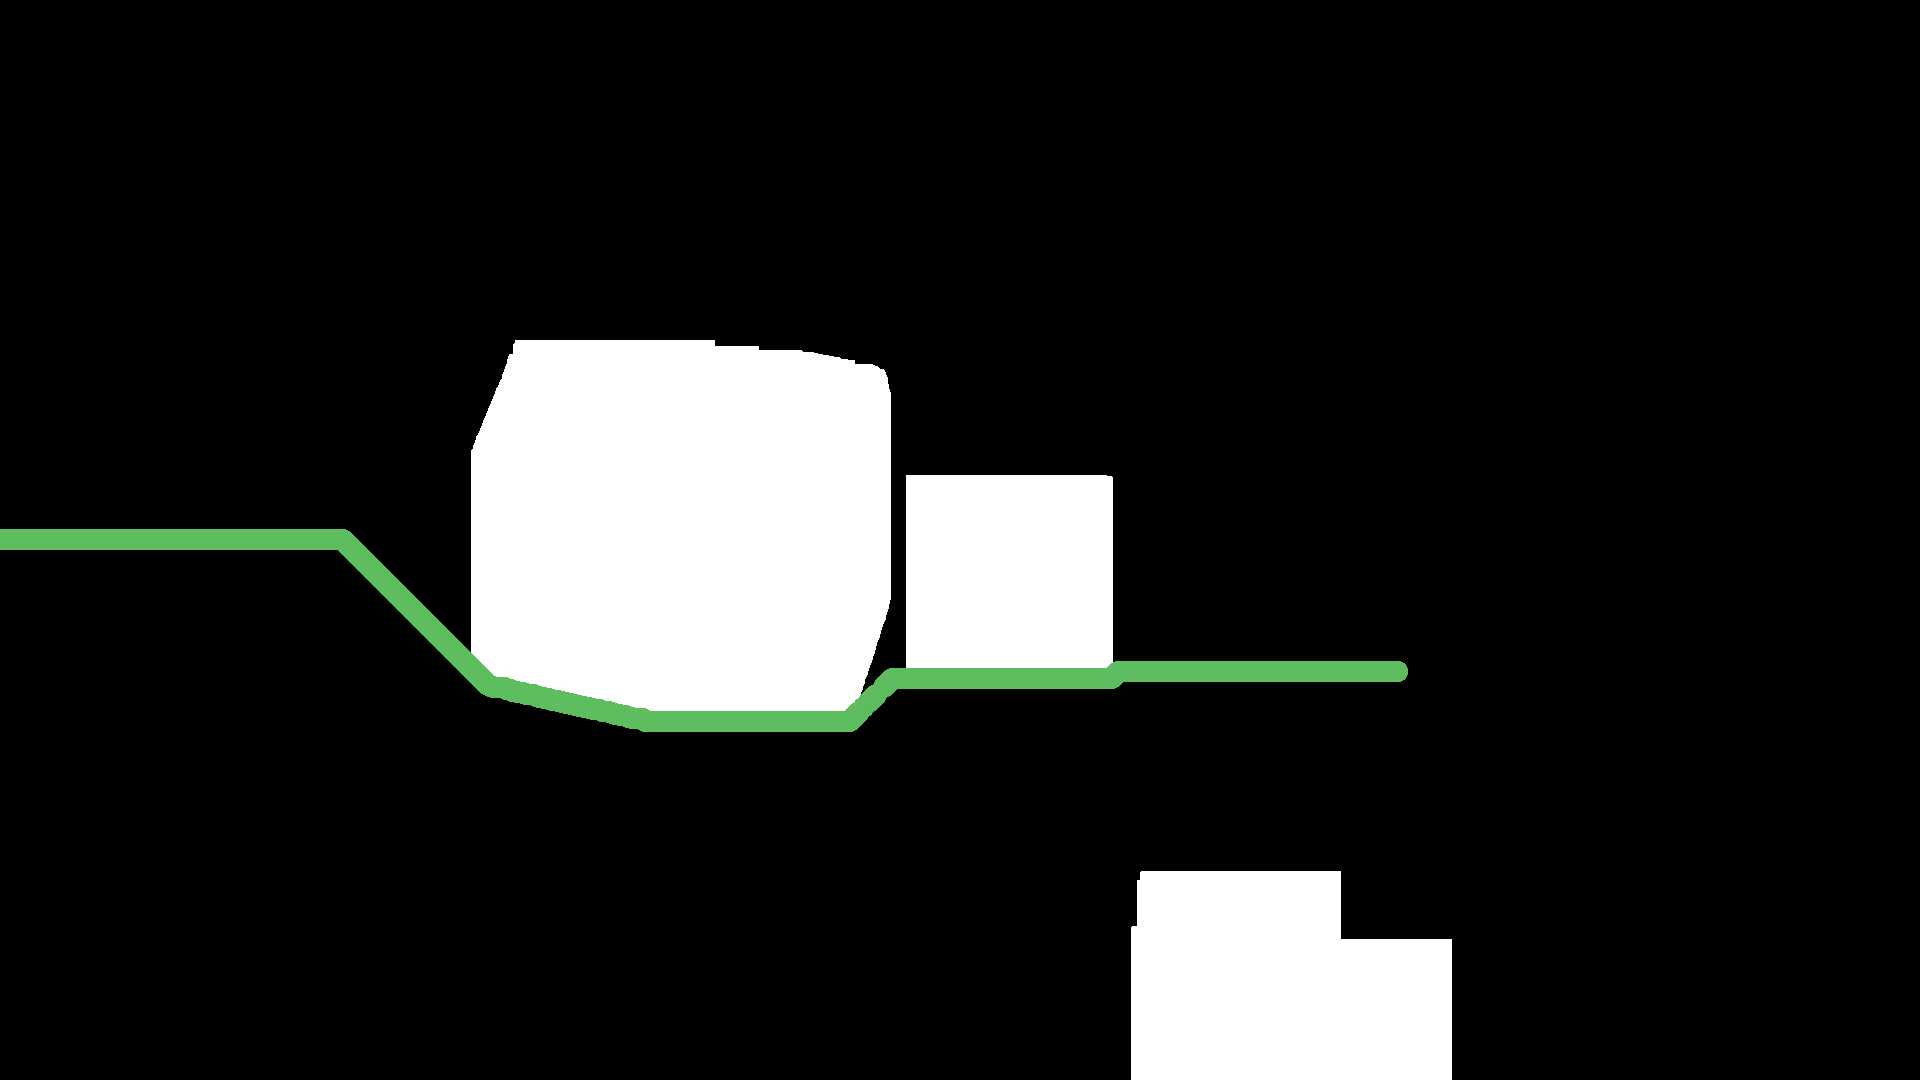
\includegraphics[width=0.49\textwidth]{./figures/path.jpeg}}
 \caption{Ejemplo del Cálculo de trayectoria}
 \label{fig:CalculoTrayectoria}
\end{figure}

\subsection{Generación de movimientos mediante datos de la trayectoria}\label{sec:GenerarMovimientos}

Se requiere un algoritmo que interprete los resultados generados por el cálculo de trayectoria y coordine los movimientos que debe ejercer el vehículo para llegar desde el origen al destino. Los movimientos se comunicarán de forma segmentada para controlar si los movimientos se realizan correctamente. Si se produce un cambio en el entorno, el coche deberá permanecer parado hasta que se calcule la nueva trayectoria.

\subsection{Comunicación con el vehículo}\label{sec:ComunicaciónVehículo}

Se necesita establecer una comunicación entre el coche y el computador del sistema para que el vehículo reciba la información correspondiente a los movimientos. Para asegurar que se sigue el camino correcto, el vehículo transmitirá mensajes de confirmación de los movimientos que vaya realizando.

\subsection{Movimiento del vehículo}\label{sec:MovimientoVehículo}

Dado que el vehículo recibirá la información correspondiente al movimiento que debe realizar, este debe extraer la información y ejecutar los movimientos de los motores en función de la orientación y la distancia que deba recorrer. Es importante que la dirección la tome con precisión, ya que de no ser así el coche podría seguir una trayectoria errónea aunque el sistema la hubiera calculado correctamente. 

\subsection{Funcionamiento del sistema en tiempo real}\label{sec:TiempoReal}

Una vez se han conseguido todos los subojetivos comentados anteriormente, se deben integrar las funcionalidades en el sistema de tal forma que se permita esquivar objetos en tiempo real. La velocidad del vehículo no es importante en este proyecto, por lo que se debe priorizar en detectar los cambios en el escenario de forma rápida y calcular la trayectoria sin que se demore mucho tiempo en el cálculo. 